\documentclass{article}

\usepackage{Sweave}
\begin{document}
\input{sample-concordance}
%\SweaveOpts{concordance=TRUE}

\title{Plant Growth \\[15pt] \large{Applied Biostatistics -- First Assignment}}
\author{Juraj Korcek \and Lucia Montero Sanchis}
\maketitle

\section{Introduction}

Your report should give a short background/introduction to the problem



\section{Exploratory Data Analysis}
2 variables:
\begin{itemize}
    \item Weight: numerical variable, continuous and positive. 
    \item Group: categorical, nominal variable. 3 categories: Control (ctrl), treatment 1 (trt1) and treatment 2 (trt2).
\end{itemize}

30 observations, 10 observations in each category of the Group variable.

\begin{figure}\label{figure:boxplots}
\begin{center}
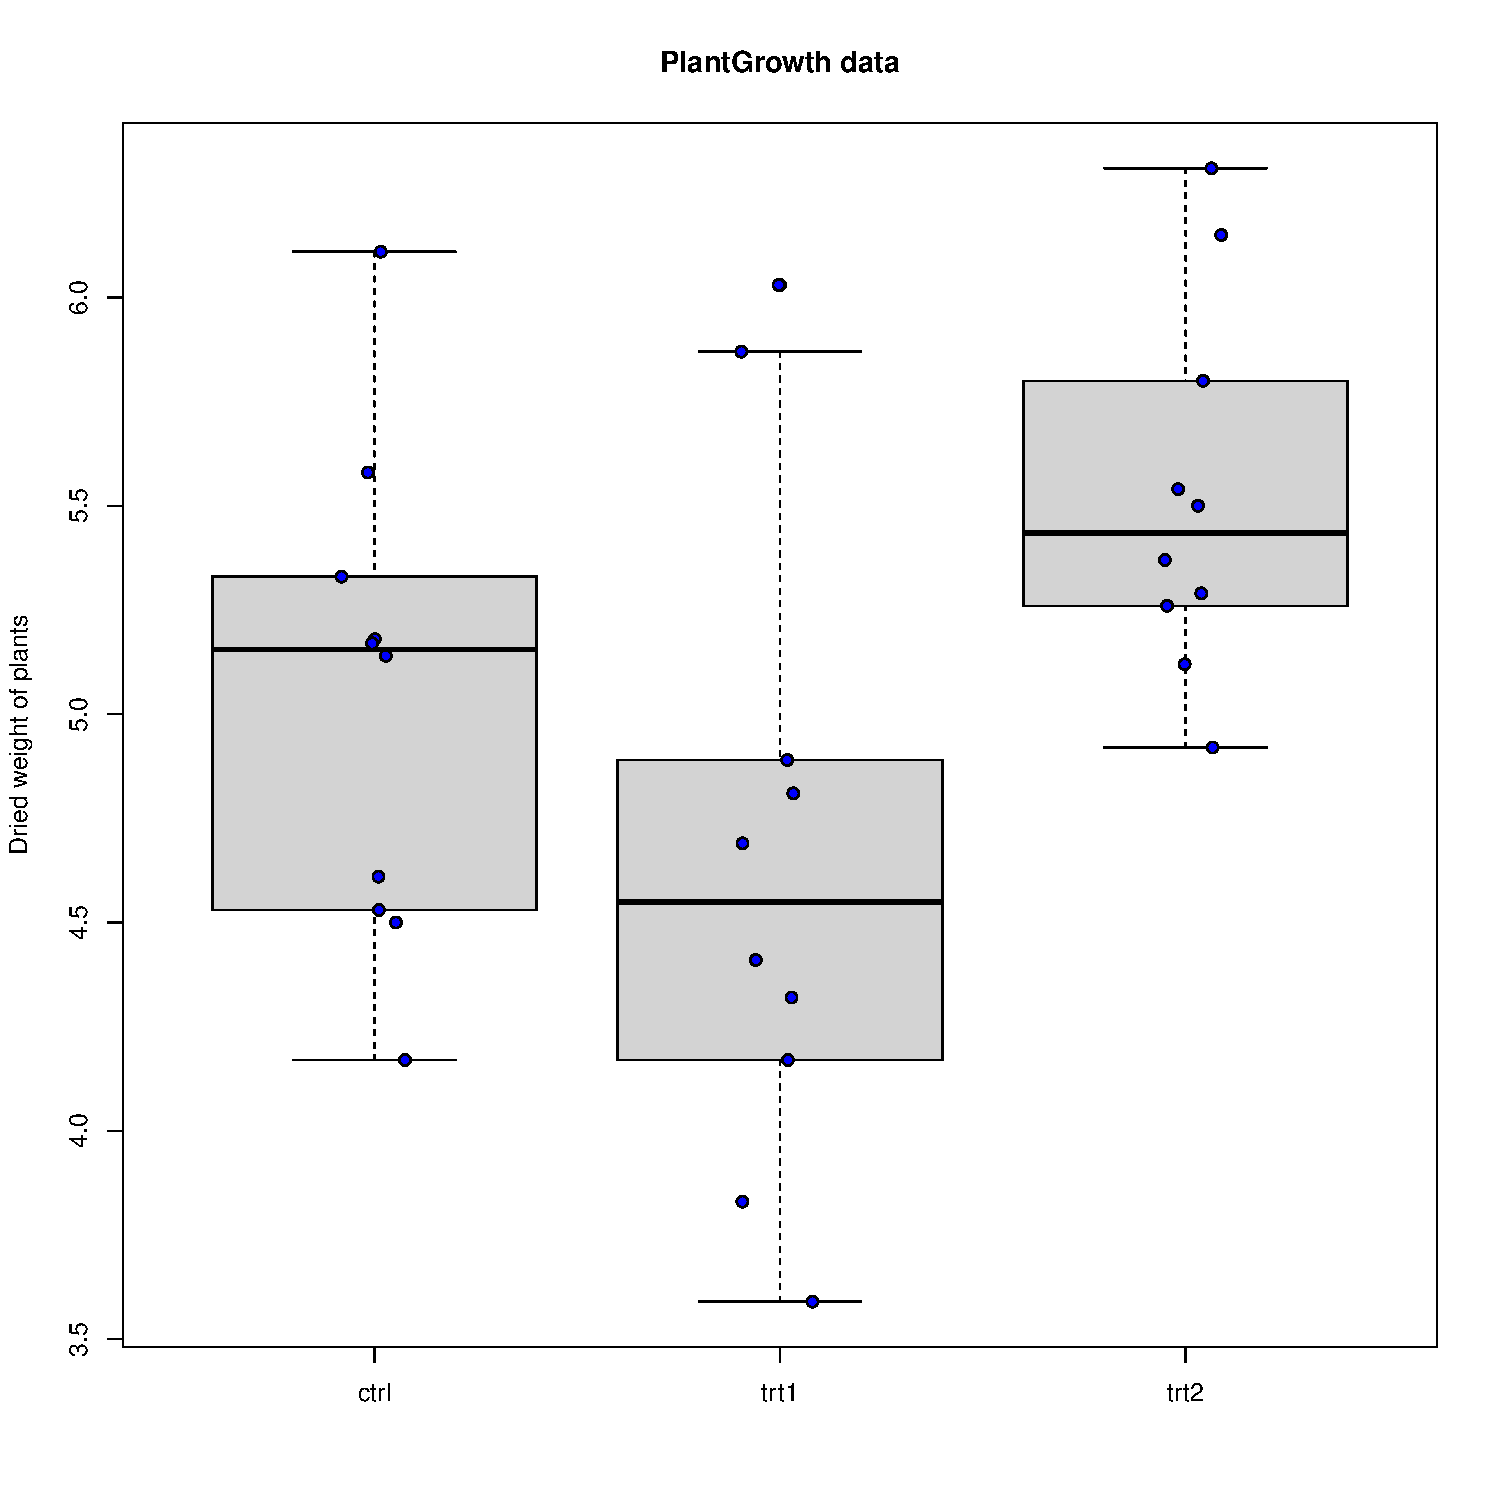
\includegraphics{sample-001}
\caption{Box plot combined with dot plot for each Group category}
\end{center}
\end{figure}



\section{Analysis of Variance}

Your report should give a description of the modeling approach and appropriate output and commentary, along with your conclusions. 



\section{Conclusions}





\end{document}

%% Table
\begin{table}[htp]\label{table:something sweet alright}
\begin{center}
